%%%%%%%%%%%%%%%%%%%%%%%%%%%%%%%%%%%%%%%%%
% a0poster Landscape Poster
% LaTeX Template
% Version 1.0 (22/06/13)
%
% The a0poster class was created by:
% Gerlinde Kettl and Matthias Weiser (tex@kettl.de)
% 
% This template has been downloaded from:
% http://www.LaTeXTemplates.com
%
% License:
% CC BY-NC-SA 3.0 (http://creativecommons.org/licenses/by-nc-sa/3.0/)
%
%%%%%%%%%%%%%%%%%%%%%%%%%%%%%%%%%%%%%%%%%

%----------------------------------------------------------------------------------------
%	PACKAGES AND OTHER DOCUMENT CONFIGURATIONS
%----------------------------------------------------------------------------------------

\documentclass[a0,landscape]{a0poster}

\usepackage{multicol} % This is so we can have multiple columns of text side-by-side
\columnsep=100pt % This is the amount of white space between the columns in the poster
\columnseprule=3pt % This is the thickness of the black line between the columns in the poster

\usepackage[svgnames]{xcolor} % Specify colors by their 'svgnames', for a full list of all colors available see here: http://www.latextemplates.com/svgnames-colors

\usepackage{times} % Use the times font
%\usepackage{palatino} % Uncomment to use the Palatino font

\usepackage{graphicx} % Required for including images
\graphicspath{{figures/}} % Location of the graphics files
\usepackage{booktabs} % Top and bottom rules for table
\usepackage[font=small,labelfont=bf]{caption} % Required for specifying captions to tables and figures
\usepackage{amsfonts, amsmath, amsthm, amssymb} % For math fonts, symbols and environments
\usepackage{wrapfig} % Allows wrapping text around tables and figures
\usepackage[T1]{fontenc}
\usepackage[utf8]{inputenc}
\usepackage{authblk}
\usepackage{color, amssymb, epsfig, graphicx, bm, amsmath, caption, subcaption, enumerate, graphicx,, setspace,listings}



\definecolor{uwred}{RGB}{197, 5, 12}

\begin{document}

%----------------------------------------------------------------------------------------
%	POSTER HEADER 
%----------------------------------------------------------------------------------------

% The header is divided into three boxes:
% The first is 55% wide and houses the title, subtitle, names and university/organization
% The second is 25% wide and houses contact information
% The third is 19% wide and houses a logo for your university/organization or a photo of you
% The widths of these boxes can be easily edited to accommodate your content as you see fit

\begin{minipage}[b]{0.55\linewidth}
\veryHuge \color{uwred} \textbf{Global PCA of Local Moments} \color{Black}\\ % Title
\Huge\textit{With Applications to MRI Segmentation}\\[1cm] % Subtitle
\huge \textbf{Jacob M. $\text{Maronge}^{\text{\large1, 2}}$, John $\text{Muschelli}^{\text{\large3}}$, Ciprian M. $\text{Crainiceanu}^{\text{\large3}}$}\\ % Author(s)
\LARGE $^{\text{\large1}}$University of Wisconsin - Madison, Department of Statistics\\
\LARGE $^{\text{\large2}}$University of Wisconsin - Madison, Department of Biostatistics and Medical Informatics\\  % University/organization
\LARGE $^{\text{\large3}}$Johns Hopkins Bloomberg School of Public Health, Department of Biostatistics
\end{minipage}
%
\begin{minipage}[b]{0.25\linewidth}
\color{DarkSlateGray}\Large \textbf{Contact Information:}\\
Jacob M. Maronge\\
Department of Statistics\\ % Address
University of Wisconsin - Madison\\
1300 University Ave, Madison, WI, 53706\\\\
Email: \texttt{jmmaronge@gmail.com}\\ % Email address
Website: \texttt{https://jmmaronge.github.io}
\end{minipage}
%
\begin{minipage}[b]{0.19\linewidth}

\includegraphics[width=23cm]{logo.png} % Logo or a photo of you, adjust its dimensions here
\end{minipage}

\vspace{1cm} % A bit of extra whitespace between the header and poster content

%----------------------------------------------------------------------------------------

\begin{multicols}{3} % This is how many columns your poster will be broken into, a poster with many figures may benefit from less columns whereas a text-heavy poster benefits from more

%----------------------------------------------------------------------------------------
%	ABSTRACT
%----------------------------------------------------------------------------------------

\color{black} % Navy color for the abstract

\normalsize{\section*{\center{\color{uwred}Abstract}}}
\hspace{1cm}We are interested in describing the information contained in local neighborhoods, and higher moments of local neighborhoods, of complex multimodal imaging techniques at the population level. This is problematic because of the size of medical imaging data. We propose a simple, computationally-efficient approach for representing the variation in multimodal images using the spatial information contained in all local neighborhoods across multiple subjects. This method achieves 3 goals: 1) decomposes the observed variability images at the population level; 2) describes and quantifies the main directions of variation; 3) uses these directions of variation to improve segmentation and studies of association with health outcomes. To achieve this, we efficiently decompose the observed variation in local neighborhood moments. In order to assess the quality of this method we show results using the 2015 Ischemic Stroke Lesion Segmentation (ISLES) Challenge.\vspace{.5cm}

%----------------------------------------------------------------------------------------
%	INTRODUCTION
%----------------------------------------------------------------------------------------

\color{black} % SaddleBrown color for the introduction
\large{\section*{\color{uwred}Introduction}}
\hspace{1cm} Every image can be vectorized. However, its meaning, interpretation, and complexity is encapsulated in the collection of all neighborhoods of all locations. More precisely, every image with $V$ voxels can be represented as a $V\times V$ matrix, where every row represents a location in the image and every column reprents a particular position in the neighborhood of that location; e.g., the first column could be the neighbor just above the location, the second column could be the neighbor to the left. Such  matrices are very large and store information inefficiently, but they provide a useful theoretical framework for representation of imaging information. Here we propose to exploit this theoretical framework to introduce simple methods to quantify the variation in multimodal images based on the shared information across local spatial neighborhoods and subjects.

\hspace{1cm}Here we consider the case when multimodal imaging is available and images are spatially co-registered within-subject, but not necessarily across subjects.  Such data are routinely available in MRI studies, where FLAIR, T1-weighted and T2-weighted images are collected for multiple subjects. Our goals are:
\begin{center}\vspace{.75cm}
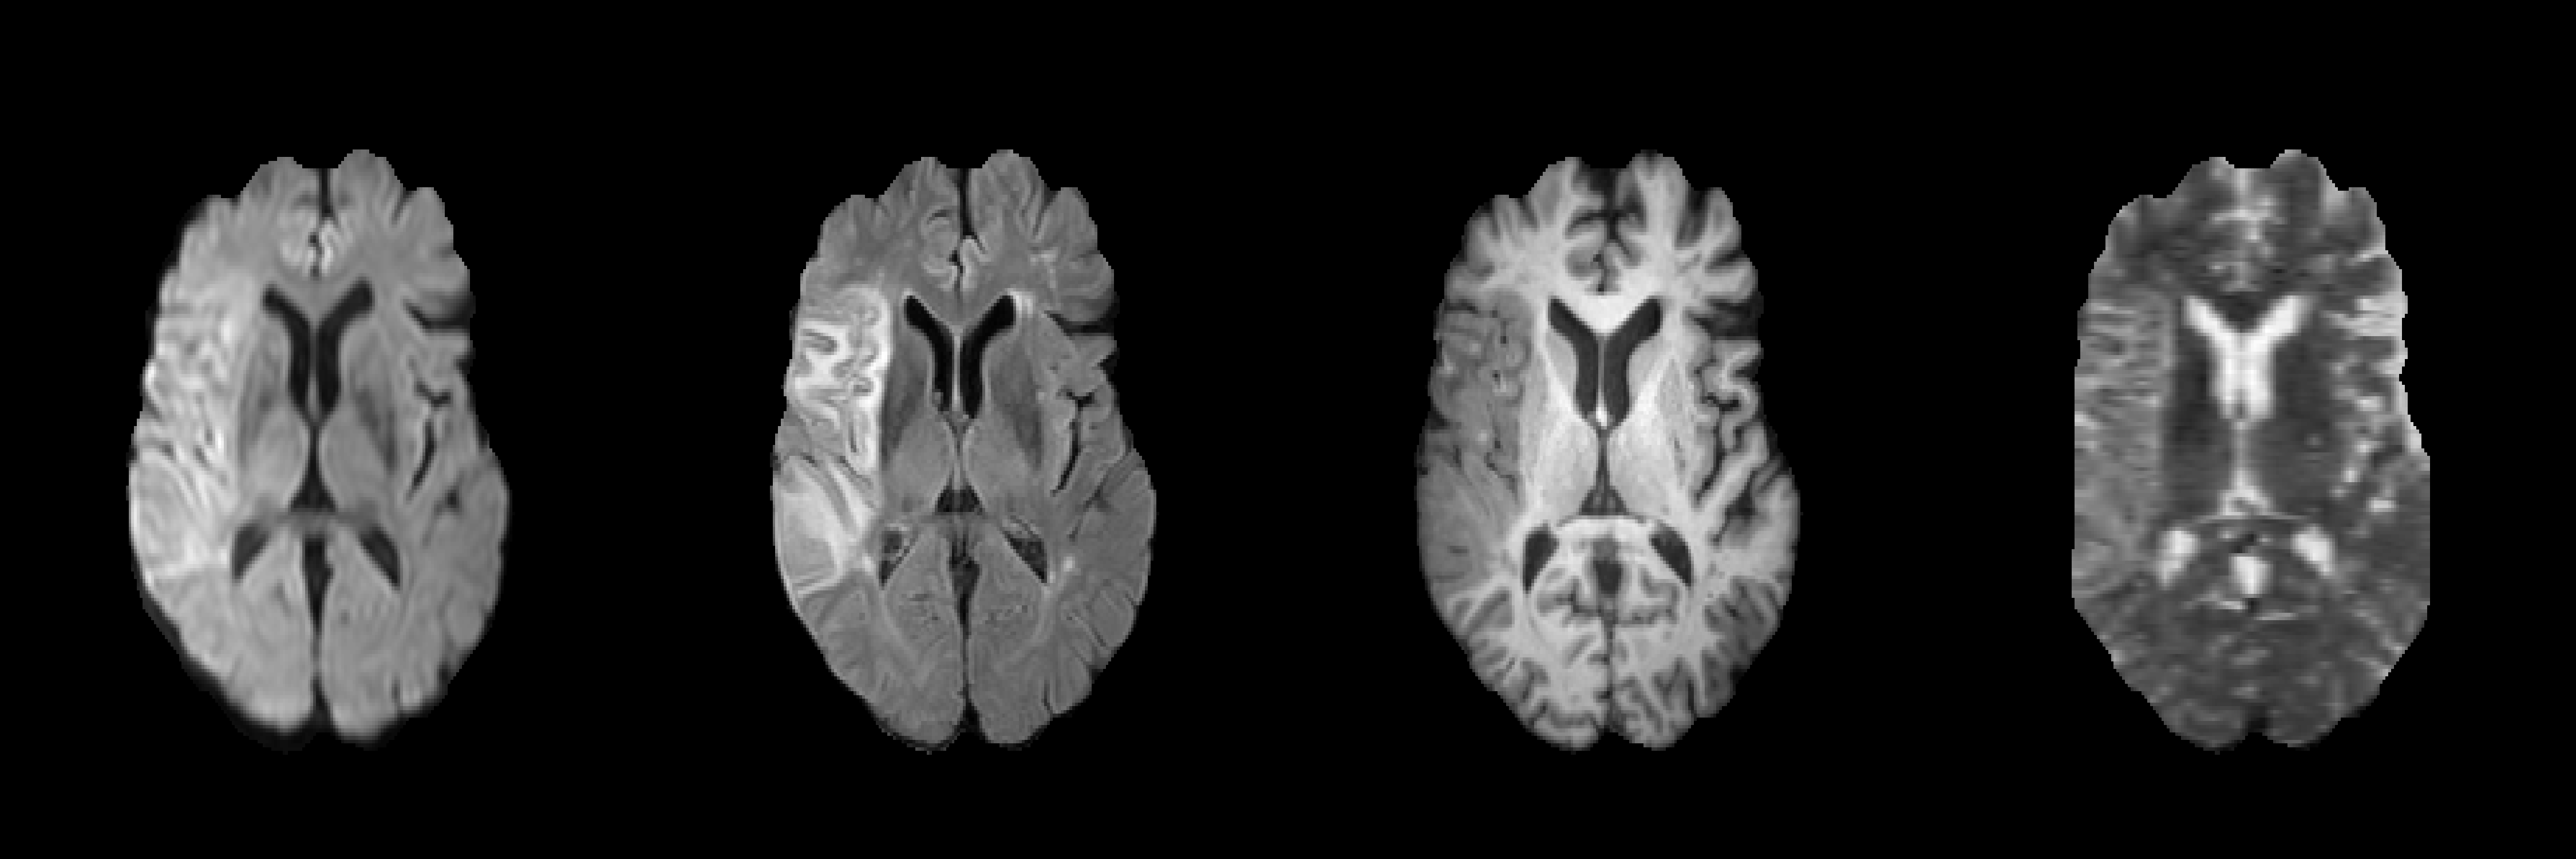
\includegraphics[width=1\linewidth]{image_ex.pdf}
\captionof{figure}{From left to right: DWI, FLAIR, T1w, and T2w images for Subject 05, 2015 ISLES Challenge}
\end{center}\vspace{.5cm}
\begin{enumerate}
\item  Decompose observed variability images at the population level
\item Describe and quantify the main directions of variation
\item Use these directions of variation to improve segmentation and studies of association with health outcomes.
\end{enumerate}


%----------------------------------------------------------------------------------------
%	MATERIALS AND METHODS
%----------------------------------------------------------------------------------------
\large{\section*{\color{uwred}Materials and Methods}}
\hspace{1cm}To achieve these objectives we propose to decompose the local variability of various moments of the image intensities: the image intensity, image  intensity square, and so on. To build intuition, consider the case when we only have one image per subject, which contains $V_i$ voxels for subject $i$, though ideas will extend to the case when there are more images.  The main idea is to represent the image as a $V_i\times K$ matrix, where every row corresponds to a voxel and contains the image intensity of the $K$ neighbors of that particular voxel given a specified ordering. For presentation and computational purposes we work with neighborhoods of size $K=27$ (adjacent neighbors only in 3D), but methods can easily be applied to any neighborhood size.  The second idea is to consider matrices obtained by taking the higher order moments of the original image and unfold them using the same procedure as the one for image intensities.  Thus, if we consider all moments up to the fourth moment then the matrix representation of the image will be $V_i\times (4K)$ dimensional.

\hspace{1cm}Consider the following mock example:
\begin{center}\vspace{.5cm}
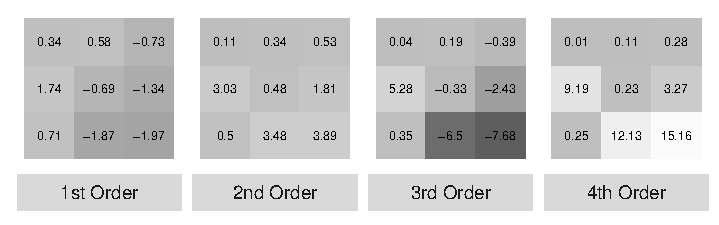
\includegraphics[width=1\linewidth]{ln_example_higherorder.pdf}
\captionof{figure}{2-D mock example of moments of local neighbors}
\end{center}\vspace{.5cm}
\normalsize{
\begin{align*}
\begin{aligned}
X_{ij} = &(0.34, 0.58, -0.73, 1.74, -0.69, -1.34, 0.71, -1.87, -1.97,\\
&0.11, 0.34, 0.53, 3.03, 0.48, 1.81, 0.50, 3.48, 3.89, \\
&0.04, 0.19, -0.39, 5.28, -0.33, -2.43, 0.35, -6.50, -7.68,\\
&0.01, 0.11, 0.28, 9.19, 0.23, 3.27, 0.25, 12.13, 15.16).
\end{aligned}
\end{align*}}
\large
\noindent This gives the $j$th row for subject $i$. If we are interested in considering additional imaging modalities, we simply add those as additional columns in the matrix. We preform this operation for each voxel for each subject and stack these vectors into a (potentially large) matrix $\mathbf{X}$.

\hspace{1cm} Once the matrix $\mathbf{X}$ is built, we center and scale each column to ensure that the observed information is not dominated by the scale of higher moments and conduct PCA. This is equivalent to conducting PCA on the correlation matrix between the columns of $\mathbf{X}$. The size of the matrix $\mathbf{X}$ is large and there is a need to use this matrix without loading it in the computer memory.

\hspace{1cm} Finally, we use the scores from the principal component analysis to fit a principal component regression model where an expert manual segmentation is the outcome. Data are separated into a training and testing set to assess performance.

\large{\section*{\color{uwred}Computational Challenges}}
\hspace{1cm}Since the size of the matrix $\mathbf{X}$ is large, we need to decompose this matrix without loading it into memory. To overcome this challenge, we iteratively read in each subject and calculate sufficient statistics for the principal component analysis of the correlation matrix between the columns of $\mathbf{X}$. This is implemented in the R package MEDALS (Memory Efficient Decomposition for Analysis of Local neighborhood moments for Segmentation) and is available at https://github.com/JMMaronge/medals.
\vspace{.5cm}
%--------------------------------------------------------------------------------------
%	RESULTS 
%----------------------------------------------------------------------------------------

\large{\section*{\color{uwred}Results}}
\hspace{1cm}Below we show partial ROC (pROC) curves for each subject, as well as overall training and overall testing results. We also show an example of how we performed on a particular subject.

\begin{center}\vspace{.5cm}
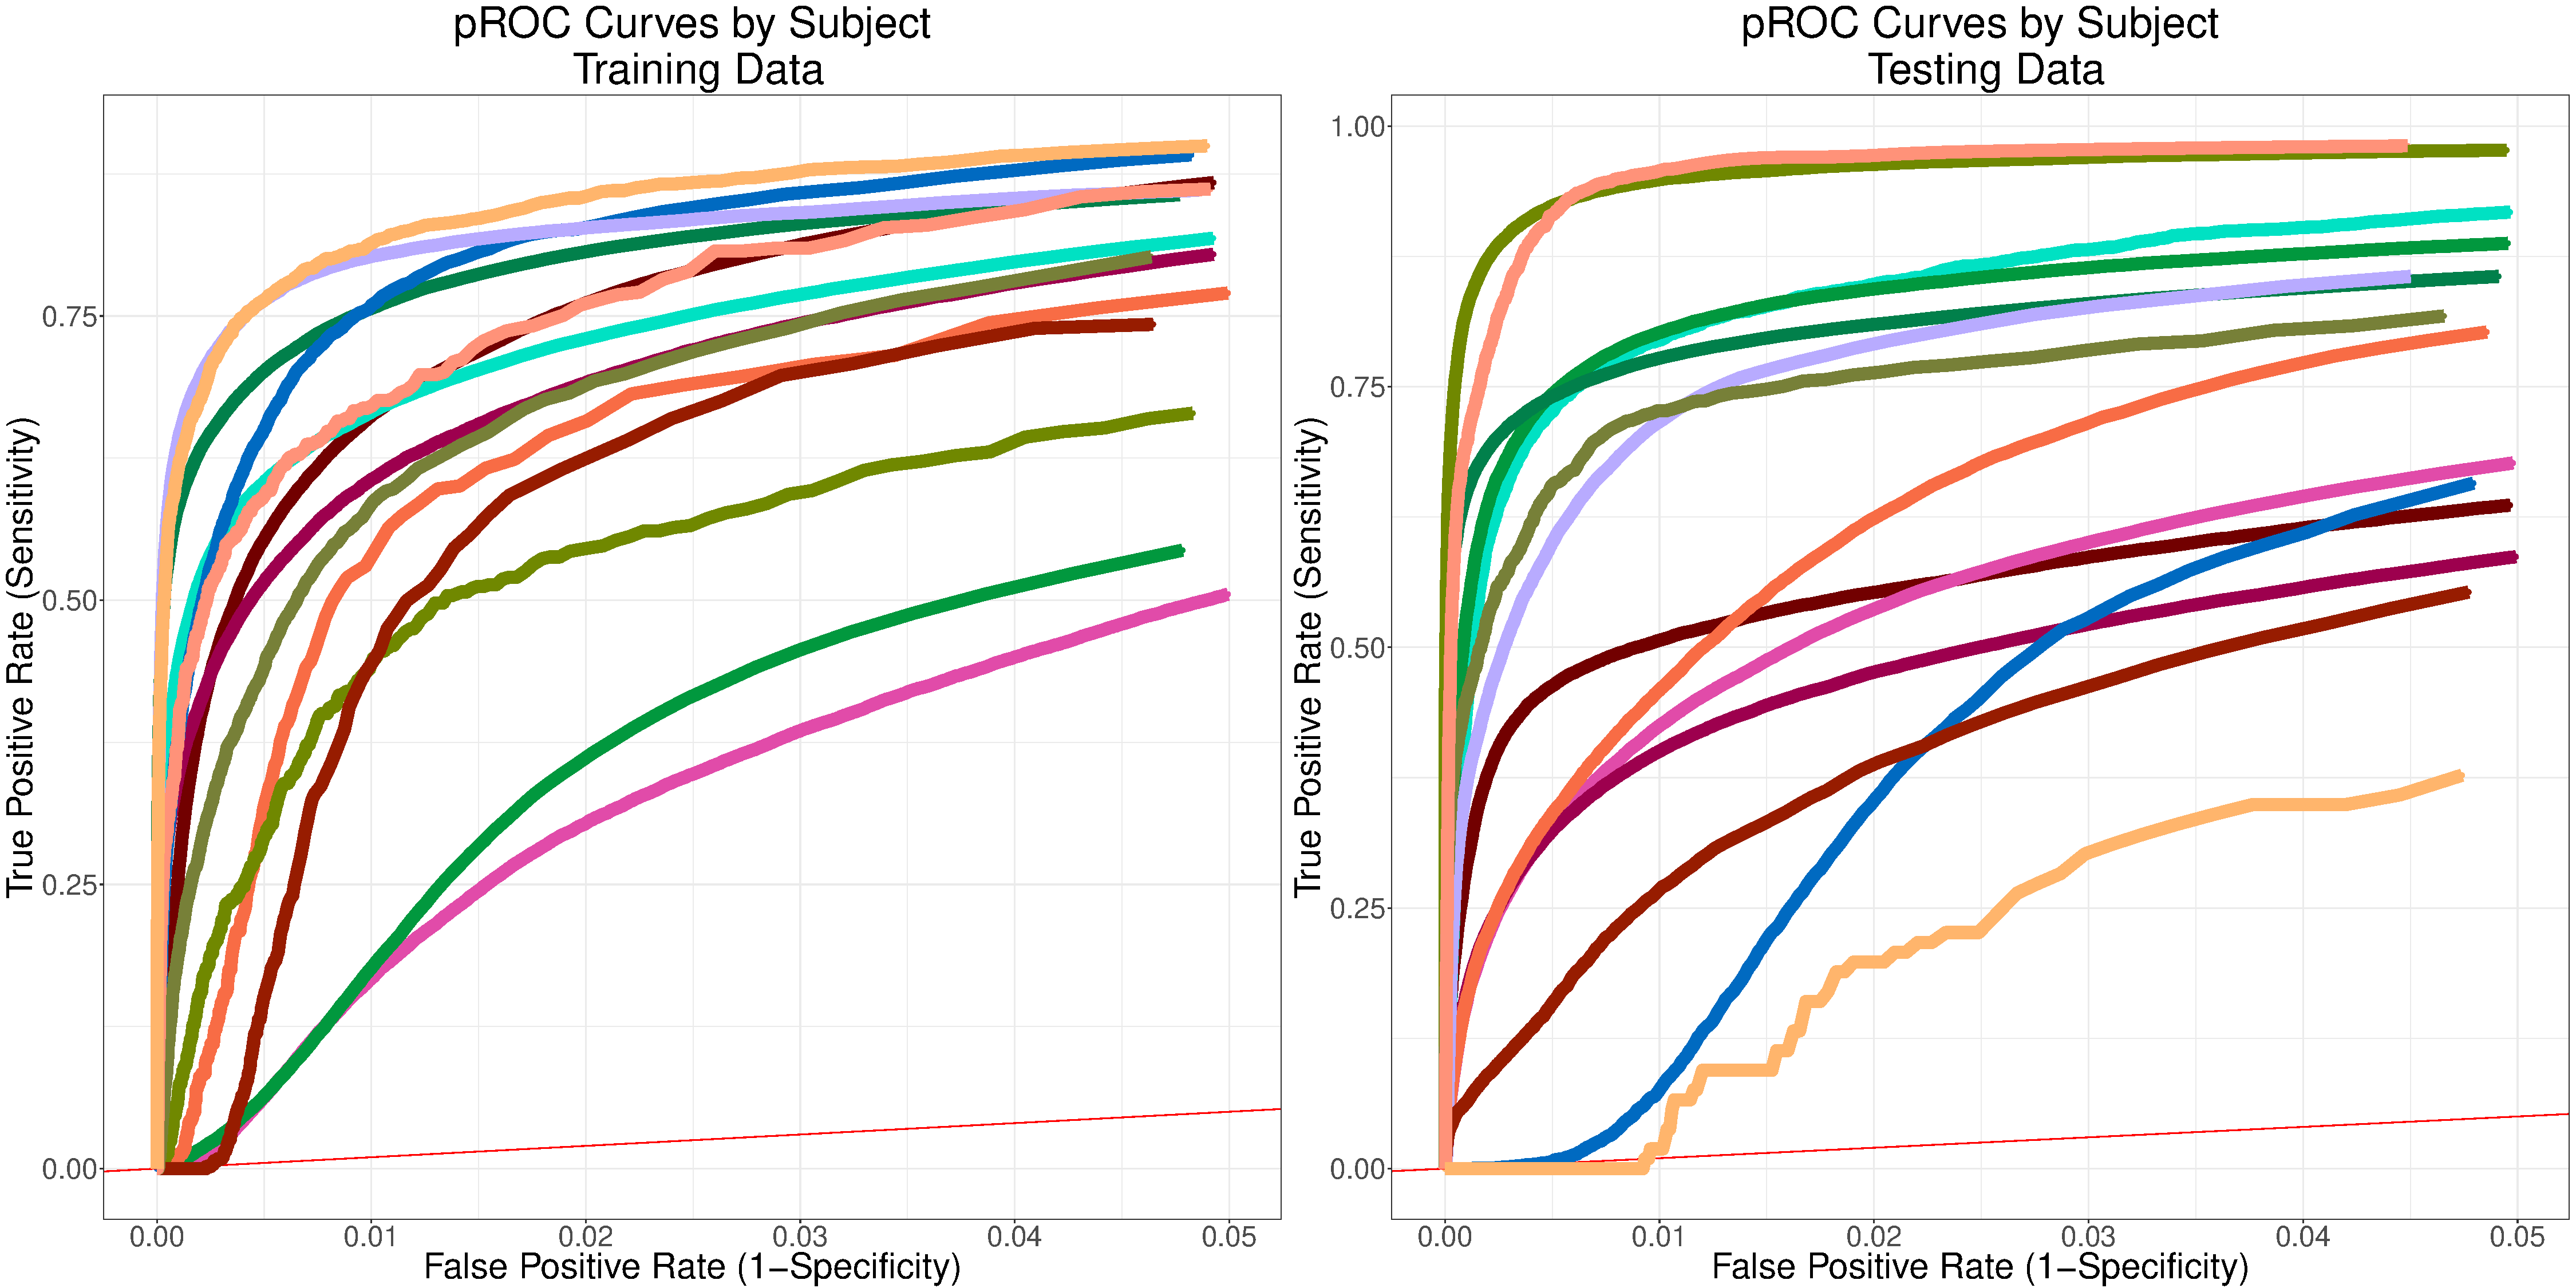
\includegraphics[width=1\linewidth]{procbysubject.pdf}
\captionof{figure}{Subject level pROC curves for training set and testing set}
\end{center}\vspace{.5cm}

\begin{center}\vspace{.5cm}
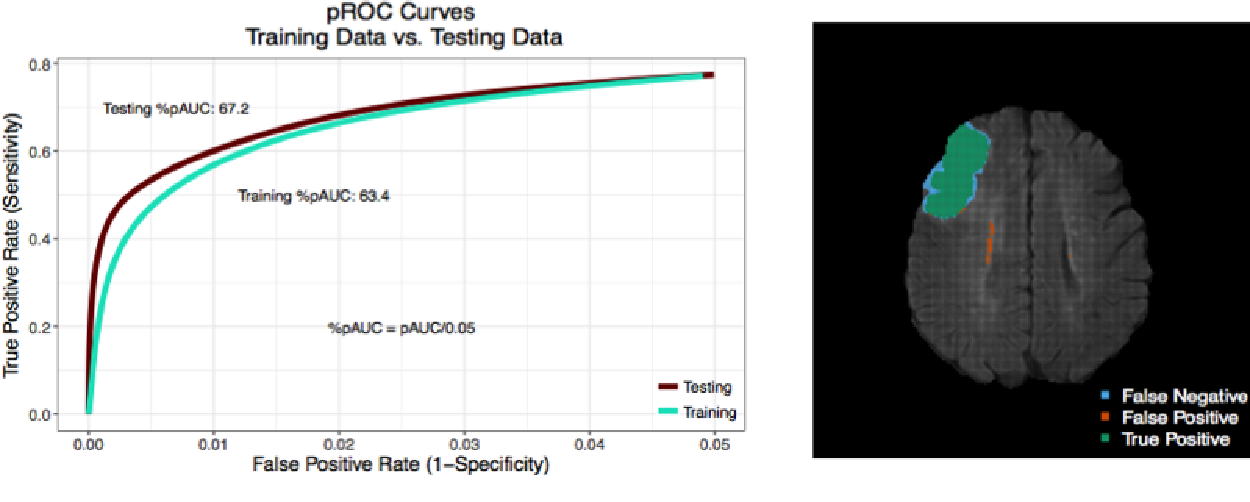
\includegraphics[width=1\linewidth]{bothplots.pdf}
\captionof{figure}{(left) Overall training results and overall testing results (right) Example of performance on one subject}
\end{center}\vspace{.5cm}

\large{\section*{\color{uwred}Conclusions}}
\hspace{1cm}In conclusion, carefully leveraging the information contained within neighborhoods appears to lead to interesting results in data applications. Future work should address how these methods compare to strictly vectorized approaches.
\end{multicols}
\end{document}

